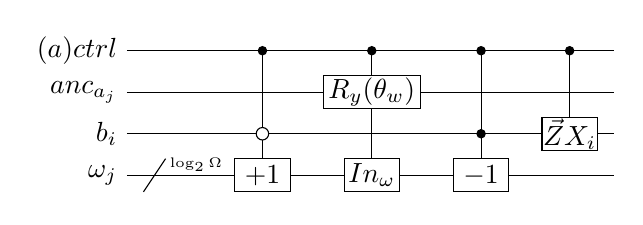
\begin{tikzpicture}[scale=1.000000,x=1pt,y=1pt]
\filldraw[color=white] (0.000000, -7.500000) rectangle (176.000000, 52.500000);
% Drawing wires
% Line 1: ctrl W \text{(a) }ctrl
\draw[color=black] (0.000000,45.000000) -- (176.000000,45.000000);
\draw[color=black] (0.000000,45.000000) node[left] {$\text{(a) }ctrl$};
% Line 2: anc_a W anc_{a_j}
\draw[color=black] (0.000000,30.000000) -- (176.000000,30.000000);
\draw[color=black] (0.000000,30.000000) node[left] {$anc_{a_j}$};
% Line 3: i W b_i
\draw[color=black] (0.000000,15.000000) -- (176.000000,15.000000);
\draw[color=black] (0.000000,15.000000) node[left] {$b_i$};
% Line 4: j W \omega_j
\draw[color=black] (0.000000,0.000000) -- (176.000000,0.000000);
\draw[color=black] (0.000000,0.000000) node[left] {$\omega_j$};
% Done with wires; drawing gates
% Line 6: j / ^{\log_2{\Omega}}
\draw (6.000000, -6.000000) -- (14.000000, 6.000000);
\draw (12.000000, 3.000000) node[right] {$\scriptstyle{^{\log_2{\Omega}}}$};
% Line 7: ctrl i anc_a j LABEL width=1
% Line 9: j G width=20 $+1$ ctrl -i
\draw (49.000000,45.000000) -- (49.000000,0.000000);
\begin{scope}
\draw[fill=white] (49.000000, -0.000000) +(-45.000000:14.142136pt and 8.485281pt) -- +(45.000000:14.142136pt and 8.485281pt) -- +(135.000000:14.142136pt and 8.485281pt) -- +(225.000000:14.142136pt and 8.485281pt) -- cycle;
\clip (49.000000, -0.000000) +(-45.000000:14.142136pt and 8.485281pt) -- +(45.000000:14.142136pt and 8.485281pt) -- +(135.000000:14.142136pt and 8.485281pt) -- +(225.000000:14.142136pt and 8.485281pt) -- cycle;
\draw (49.000000, -0.000000) node {$+1$};
\end{scope}
\filldraw (49.000000, 45.000000) circle(1.500000pt);
\draw[fill=white] (49.000000, 15.000000) circle(2.250000pt);
% Line 10: anc_a G:width=35 $R_y(\theta_w)$ j G:width=20 $In_\omega$ ctrl
\draw (88.500000,45.000000) -- (88.500000,0.000000);
\begin{scope}
\draw[fill=white] (88.500000, 30.000000) +(-45.000000:24.748737pt and 8.485281pt) -- +(45.000000:24.748737pt and 8.485281pt) -- +(135.000000:24.748737pt and 8.485281pt) -- +(225.000000:24.748737pt and 8.485281pt) -- cycle;
\clip (88.500000, 30.000000) +(-45.000000:24.748737pt and 8.485281pt) -- +(45.000000:24.748737pt and 8.485281pt) -- +(135.000000:24.748737pt and 8.485281pt) -- +(225.000000:24.748737pt and 8.485281pt) -- cycle;
\draw (88.500000, 30.000000) node {$R_y(\theta_w)$};
\end{scope}
\begin{scope}
\draw[fill=white] (88.500000, -0.000000) +(-45.000000:14.142136pt and 8.485281pt) -- +(45.000000:14.142136pt and 8.485281pt) -- +(135.000000:14.142136pt and 8.485281pt) -- +(225.000000:14.142136pt and 8.485281pt) -- cycle;
\clip (88.500000, -0.000000) +(-45.000000:14.142136pt and 8.485281pt) -- +(45.000000:14.142136pt and 8.485281pt) -- +(135.000000:14.142136pt and 8.485281pt) -- +(225.000000:14.142136pt and 8.485281pt) -- cycle;
\draw (88.500000, -0.000000) node {$In_\omega$};
\end{scope}
\filldraw (88.500000, 45.000000) circle(1.500000pt);
% Line 11: j G width=20 $-1$ ctrl i
\draw (128.000000,45.000000) -- (128.000000,0.000000);
\begin{scope}
\draw[fill=white] (128.000000, -0.000000) +(-45.000000:14.142136pt and 8.485281pt) -- +(45.000000:14.142136pt and 8.485281pt) -- +(135.000000:14.142136pt and 8.485281pt) -- +(225.000000:14.142136pt and 8.485281pt) -- cycle;
\clip (128.000000, -0.000000) +(-45.000000:14.142136pt and 8.485281pt) -- +(45.000000:14.142136pt and 8.485281pt) -- +(135.000000:14.142136pt and 8.485281pt) -- +(225.000000:14.142136pt and 8.485281pt) -- cycle;
\draw (128.000000, -0.000000) node {$-1$};
\end{scope}
\filldraw (128.000000, 45.000000) circle(1.500000pt);
\filldraw (128.000000, 15.000000) circle(1.500000pt);
% Line 13: i G width=20 $\vec{Z}X_i$ ctrl
\draw (160.000000,45.000000) -- (160.000000,15.000000);
\begin{scope}
\draw[fill=white] (160.000000, 15.000000) +(-45.000000:14.142136pt and 8.485281pt) -- +(45.000000:14.142136pt and 8.485281pt) -- +(135.000000:14.142136pt and 8.485281pt) -- +(225.000000:14.142136pt and 8.485281pt) -- cycle;
\clip (160.000000, 15.000000) +(-45.000000:14.142136pt and 8.485281pt) -- +(45.000000:14.142136pt and 8.485281pt) -- +(135.000000:14.142136pt and 8.485281pt) -- +(225.000000:14.142136pt and 8.485281pt) -- cycle;
\draw (160.000000, 15.000000) node {$\vec{Z}X_i$};
\end{scope}
\filldraw (160.000000, 45.000000) circle(1.500000pt);
% Done with gates; drawing ending labels
% Done with ending labels; drawing cut lines and comments
% Done with comments
\end{tikzpicture}
